% =============================================================
%  Test document: TikZ single-line diagram of a cable link
%  Combines the two test folders, documentation/test (plain TikZ
%  figure in the report template) and presentation/test (circuitikz
%  figure in a beamer frame), into one report.
%  Uses the shared American Terawatt report style.
%  Compile:  pdflatex transmission-line.tex   (run twice)
% =============================================================
\documentclass[11pt,a4paper]{article}

% Shared style lives in the repo-level template folder. This document
% sits one level below the repository root rather than the usual two,
% so the template path is declared before the package is loaded.
\providecommand{\attemplatepath}{../template/}
\usepackage[corporate]{../template/attemplate}

% The circuitikz variant of the figure needs these; the plain TikZ
% variant needs only arrows.meta and calc.
\usepackage{circuitikz}
\usetikzlibrary{arrows.meta,calc,decorations.pathreplacing}

\newcommand{\cmd}[1]{\texttt{\small #1}}

% ---- Report metadata ----------------------------------------
\reporttitle{Cable Link Single-Line Diagram4}
\reportsubtitle{TikZ and circuitikz renderings of the sending-end / receiving-end transmission model}
\atEyebrow{Template test}
\atAbstract{Test document for the shared report template, combining the
two earlier test folders. It compiles both renderings of the single-line
diagram of a cable transmission link (source, disconnectors, cable of
length $L_{\mathrm{cable}}$ and load impedance $Z_{L}$) with the
sending-end and receiving-end voltages, currents and power flows, and
checks them against the original drawing.}
\reportauthor{Eugen Starschich}
\reportdocnumber{ATW-TST-TIKZ-001}
\reportrevision{0.2}
\reportstatus{Draft}
\reportdate{\today}
\reportconfidentiality{Internal}

\begin{document}

\makecover

\revisionhistory{
  \revrow{0.1}{Sep. 18, 2026}{Eugen Starschich}{Initial document}
  \revrow{0.2}{Sep. 18, 2026}{Eugen Starschich}{\cmd{documentation/test} and \cmd{presentation/test} combined in \cmd{test/}; circuitikz variant added}
}

\clearpage

\section{Comparison with the original}

Figure~\ref{fig:transmission-line-original} reproduces the original
drawing (\cmd{figures/image9.pdf}) that the TikZ figure was traced
from, for a side-by-side check of geometry, colours and labels. Both
figures are scaled to the full text width, so they can be compared
directly.

\begin{figure}[!ht]
  \centering
  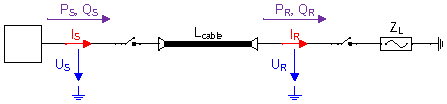
\includegraphics[width=\linewidth]{figures/image9.pdf}
  \caption{Original drawing used as reference.}
  \label{fig:transmission-line-original}
\end{figure}

\begin{figure}[!ht]
  \centering
  \resizebox{\linewidth}{!}{% -------------------------------------------------------------
%  Single-line diagram of a cable transmission link
%  TikZ rendering of image9.pdf (sending end S, cable, receiving
%  end R with load impedance Z_L). Include with \input{...} inside
%  a figure environment; tikz is loaded by the shared template.
%  Requires: \usetikzlibrary{arrows.meta}
% -------------------------------------------------------------
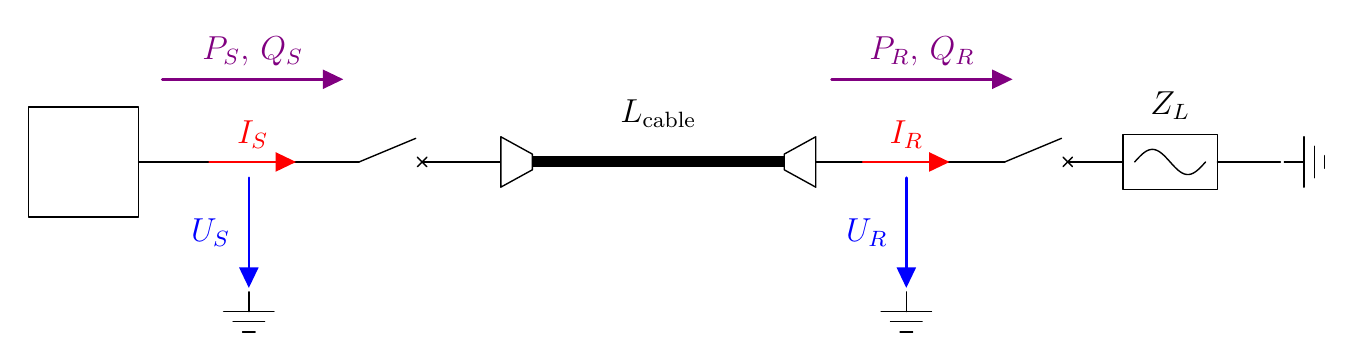
\begin{tikzpicture}[
  line cap=round, line join=round,
  wire/.style={draw=black, line width=0.5pt},
  cable/.style={draw=black, line width=4pt, line cap=butt},
  current/.style={draw=red,    line width=0.9pt, -{Triangle[length=2.6mm,width=2.4mm]}},
  voltage/.style={draw=blue,   line width=0.9pt, -{Triangle[length=2.6mm,width=2.4mm]}},
  power/.style={draw=violet,   line width=0.9pt, -{Triangle[length=2.6mm,width=2.4mm]}},
  lbl/.style={font=\sffamily\large},
  % ground symbol: three bars of decreasing width, anchored at the top
  pics/ground/.style={code={
      \draw[wire] (0,0) -- (0,-0.25);
      \draw[wire] (-0.32,-0.25) -- (0.32,-0.25);
      \draw[wire] (-0.20,-0.38) -- (0.20,-0.38);
      \draw[wire] (-0.08,-0.51) -- (0.08,-0.51);
  }},
  % open disconnector: contacts at (0,0) and (0.8,0)
  pics/switch/.style={code={
      \draw[wire] (0,0) -- (0.72,0.30);
      \draw[wire] (0.74,-0.06) -- (0.86,0.06);
      \draw[wire] (0.74,0.06) -- (0.86,-0.06);
      \draw[wire] (0.8,0) -- (0.95,0);
  }},
]
  % ---- sending end -------------------------------------------
  \draw[wire] (0,-0.7) rectangle (1.4,0.7);          % source / converter block
  \draw[wire] (1.4,0) -- (4.2,0);
  \draw[current] (2.3,0) -- (3.4,0) node[midway, above=1pt, lbl, red] {$I_{S}$};
  \draw[voltage] (2.8,-0.2) -- (2.8,-1.6) node[midway, left=3pt, lbl, blue] {$U_{S}$};
  \pic[blue] at (2.8,-1.65) {ground};
  \draw[power] (1.7,1.05) -- (4.0,1.05) node[midway, above=1pt, lbl, violet] {$P_{S},\,Q_{S}$};

  % ---- sending-end disconnector ------------------------------
  \pic at (4.2,0) {switch};
  \draw[wire] (5.15,0) -- (6.0,0);

  % ---- cable with terminations -------------------------------
  \draw[wire, fill=white] (6.0,-0.32) -- (6.0,0.32) -- (6.4,0.10) -- (6.4,-0.10) -- cycle;
  \draw[cable] (6.4,0) -- (9.6,0);
  \draw[wire, fill=white] (10.0,-0.32) -- (10.0,0.32) -- (9.6,0.10) -- (9.6,-0.10) -- cycle;
  \node[above=6pt, lbl] at (8.0,0.1) {$L_{\mathrm{cable}}$};

  % ---- receiving end -----------------------------------------
  \draw[wire] (10.0,0) -- (12.4,0);
  \draw[current] (10.6,0) -- (11.7,0) node[midway, above=1pt, lbl, red] {$I_{R}$};
  \draw[voltage] (11.15,-0.2) -- (11.15,-1.6) node[midway, left=3pt, lbl, blue] {$U_{R}$};
  \pic[blue] at (11.15,-1.65) {ground};
  \draw[power] (10.2,1.05) -- (12.5,1.05) node[midway, above=1pt, lbl, violet] {$P_{R},\,Q_{R}$};

  % ---- receiving-end disconnector and load -------------------
  \pic at (12.4,0) {switch};
  \draw[wire] (13.35,0) -- (13.9,0);
  \draw[wire] (13.9,-0.35) rectangle (15.1,0.35);     % load impedance Z_L
  \draw[wire, domain=0:1, samples=40, smooth, variable=\t]
        plot ({14.05+0.9*\t}, {0.16*sin(360*\t)});
  \node[above=2pt, lbl] at (14.5,0.35) {$Z_{L}$};
  \draw[wire] (15.1,0) -- (15.9,0);
  \pic[rotate=90] at (15.95,0) {ground};              % ground drawn sideways
\end{tikzpicture}
}
  \caption{TikZ rendering of Figure~\ref{fig:transmission-line-original} with Fable.}
  \label{fig:transmission-line-tikz}
\end{figure}

\begin{figure}[!ht]
  \centering
  \resizebox{0.9\linewidth}{!}{% -------------------------------------------------------------
%  Single-line diagram of a cable transmission link -- circuitikz
%  variant, taken from the beamer test file
%  presentation/test/transmission-line-tikZ.tex. Include with
%  \input{...} inside a figure environment.
%  Requires: \usepackage{circuitikz}
%            \usetikzlibrary{decorations.pathreplacing}
% -------------------------------------------------------------
\begin{circuitikz}[american voltages, scale=1.2]
% Source box
\draw (0,0) rectangle (1,1);

% Label above source (P_S, Q_S)
\draw[->,violet, thick] (1,1.3) -- (3,1.3) node[midway, above] {$P_S, Q_S$};

% Line from source to point S
\draw (1,0.5) -- (2,0.5);

% Point S (red dot)
\fill[red] (2,0.5) circle (2pt);
\node[right] at (2,0.6) {$S$};

% I_S arrow (red, going right)
\draw[->,red, thick] (2,0.5) -- (2.8,0.5) node[midway, above] {$I_S$};

% U_S arrow (blue, going down)
\draw[->,blue, thick] (2,0.5) -- (2,-0.5) node[midway, right] {$U_S$};

% Switch/open
\draw[thick] (3,0.5) -- (3.3,0.5);
\draw[thick] (3.3,0.5) -- (3.5,0.6) -- (3.5,0.4) -- (3.8,0.5);

% Cable (thick black line) with brace
\draw[ultra thick] (3.8,0.5) -- (6,0.5);
\draw[decorate,decoration={brace,amplitude=6pt}, above] 
    (3.8,0.5) -- (6,0.5) node[midway,above=8pt] {$L_{\text{cable}}$};

% Point R (red dot)
\fill[red] (6,0.5) circle (2pt);
\node[right] at (6,0.6) {$R$};

% I_R arrow (red, going right)
\draw[->,red, thick] (6,0.5) -- (6.8,0.5) node[midway, above] {$I_R$};

% U_R arrow (blue, going down)
\draw[->,blue, thick] (6,0.5) -- (6,-0.5) node[midway, right] {$U_R$};

% Label above point R (P_R, Q_R)
\draw[->,violet, thick] (6,1.3) -- (8,1.3) node[midway, above] {$P_R, Q_R$};

% Switch/open
\draw[thick] (6.8,0.5) -- (7.2,0.5);
\draw[thick] (7.2,0.5) -- (7.5,0.6) -- (7.5,0.4) -- (7.8,0.5);

% Load Z_L
\draw (7.8,0.5) to[R, l^=$Z_L$] (7.8,-1) node[ground]{};

% Ground from cable
\draw (6,-0.5) -- (6,-1) node[ground]{};
\draw (2,-0.5) -- (2,-1) node[ground]{};
  \end{circuitikz}
}
  \caption{TikZ rendering of Figure~\ref{fig:transmission-line-original} with qwen3.5:122b-a10b.}
  \label{fig:transmission-line-circuitikz}
\end{figure}

The two renderings differ in what they delegate to a package rather than
in what they show.






\end{document}
